%%%%%%%%%%%%%%%%%%%%%%%%%%%%%%%%%%%%%%%%%
% Beamer Presentation
% LaTeX Template
% Version 1.0 (10/11/12)
%
% This template has been downloaded from:
% http://www.LaTeXTemplates.com
%
% License:
% CC BY-NC-SA 3.0 (http://creativecommons.org/licenses/by-nc-sa/3.0/)
%
%%%%%%%%%%%%%%%%%%%%%%%%%%%%%%%%%%%%%%%%%

%----------------------------------------------------------------------------------------
%	PACKAGES AND THEMES
%----------------------------------------------------------------------------------------

\documentclass{beamer}

\mode<presentation> {

% The Beamer class comes with a number of default slide themes
% which change the colors and layouts of slides. Below this is a list
% of all the themes, uncomment each in turn to see what they look like.

%\usetheme{default}
%\usetheme{AnnArbor}
%\usetheme{Antibes}
%\usetheme{Bergen}
%\usetheme{Berkeley}
%\usetheme{Berlin}
%\usetheme{Boadilla}
\usetheme{CambridgeUS}
%\usetheme{Copenhagen}
%\usetheme{Darmstadt}
%\usetheme{Dresden}
%\usetheme{Frankfurt}
%\usetheme{Goettingen}
%\usetheme{Hannover}
%\usetheme{Ilmenau}
%\usetheme{JuanLesPins}
%\usetheme{Luebeck}
%\usetheme{Madrid}
%\usetheme{Malmoe}
%\usetheme{Marburg}
%\usetheme{Montpellier}
%\usetheme{PaloAlto}
%\usetheme{Pittsburgh}
%\usetheme{Rochester}
%\usetheme{Singapore}
%\usetheme{Szeged}
%\usetheme{Warsaw}

% As well as themes, the Beamer class has a number of color themes
% for any slide theme. Uncomment each of these in turn to see how it
% changes the colors of your current slide theme.

%\usecolortheme{albatross}
%\usecolortheme{beaver}
%\usecolortheme{beetle}
%\usecolortheme{crane}
%\usecolortheme{dove}
%\usecolortheme{fly}
%\usecolortheme{seagull}
%\usecolortheme{wolverine}
%Outer color themes
%\usecolortheme{dolphin}
%\usecolortheme{seahorse}
%\usecolortheme{whale}
%Inner color themes
%\usecolortheme{lily}
%\usecolortheme{orchid}
%\usecolortheme{rose}

%\setbeamertemplate{footline} % To remove the footer line in all slides uncomment this line
%\setbeamertemplate{footline}[page number] % To replace the footer line in all slides with a simple slide count uncomment this line

%\setbeamertemplate{navigation symbols}{} % To remove the navigation symbols from the bottom of all slides uncomment this line
}

\usepackage{gensymb}
%\usepackage{multimedia}
\usepackage{media9} 
\usepackage{graphicx} % Allows including images
\usepackage{booktabs} % Allows the use of \toprule, \midrule and \bottomrule in tables

%----------------------------------------------------------------------------------------
%	TITLE PAGE
%----------------------------------------------------------------------------------------

% The short title appears at the bottom of every slide, the full title is only on the title page
\title[Speech Recognition]{Speech Recognition Using Linear Predictive Coding and Support Vector Machines}

\author{David McNeil} % Your name
\institute[RHIT] % Your institution as it will appear on the bottom of every slide, may be shorthand to save space
{
Rose-Hulman Institute of Technology \\ % Your institution for the title page
\medskip
\textit{mcneilde@rose-hulman.edu} % Your email address
}
%\date{\today} % Date, can be changed to a custom date
\date{}

\begin{document}

% Print the title page as the first slide
\begin{frame}
\titlepage
\end{frame}

% Table of contents slide, comment this block out to remove it
\begin{frame}
\frametitle{Overview}
\tableofcontents % Throughout your presentation, if you choose to use \section{} and \subsection{} commands, these will automatically be printed on this slide as an overview of your presentation
\end{frame}

%----------------------------------------------------------------------------------------
%	PRESENTATION SLIDES
%----------------------------------------------------------------------------------------
% slides are 3in high by 5in wide
%------------------------------------------------
\section{Introduction} 
%------------------------------------------------

\begin{frame}
\frametitle{Objective}
\begin{block}{Successfully be able to distinguish samples of speech.}
\begin{itemize}
	\item Feature Extraction-- Extracting a unique set of features from the audio sample
	\item Classification-- Comparing the extracted features to the features from a known database of samples
\end{itemize}
\end{block}
\end{frame}

%------------------------------------------------

\begin{frame}
\frametitle{Create a Training Database}
\begin{block}{I created a program to record audio samples in order to build up a training database of audio samples}
\begin{itemize}
	\item 44100Hz sample rate
	\item 16 bits per sample
	\item Single channel of audio
	\item 2 second duration % Duration of recording
	\item Relatively low level of background noise
\end{itemize}
\end{block}
\end{frame}

%------------------------------------------------
\section{Feature Extraction} 
%------------------------------------------------

\begin{frame}
\frametitle{Linear Predictive Coding (LPC)}
\begin{block}{}
\begin{itemize}
	\item General filter difference equation: 
	$$y(n) = \sum_{j=1}^{N} a_j \cdot y(n-j) + \sum_{j=0}^{M} b_j \cdot x(n-j)$$
	\item $y(n)$ is predicted from past outputs and present and past inputs
	\item Use all pole filter model 
	\begin{itemize}
		\item $M = 0$
		\item Prediction based only on past outputs and the current input
	\end{itemize} 
\end{itemize}
\end{block}
\end{frame}

%------------------------------------------------

\begin{frame}
\frametitle{Linear Predictive Coding (LPC)}
\begin{block}{}
\begin{itemize}
	\item Estimation of output: 
	$$\hat{y}(n) = \sum_{j=1}^{N} a_j \cdot y(n-j))$$
	\item Prediction error: 
	$e(n) = y(n) - \hat{y}(n)$
\end{itemize}
\end{block}
\end{frame}

%------------------------------------------------

\begin{frame}
\frametitle{Linear Predictive Coding (LPC)}
\begin{block}{}
\begin{itemize}
	\item Solve for $y(n)$ and plug in definition for $\hat{y}(n)$: 
	$$y(n) = \sum_{j=1}^{N} a_j \cdot y(n-j) + e(n)$$
	\item All pole filter model:
	$$y(n) = \sum_{j=1}^{N} a_j \cdot y(n-j) + b_0 \cdot x(n)$$
	\item By comparison $e(n) = b_0 \cdot x(n)$
	\item The prediction error is a result of the input (filter excitation source)
\end{itemize}
\end{block}
\end{frame}

%------------------------------------------------

\begin{frame}
\frametitle{Linear Predictive Coding (LPC)}
\begin{block}{}
\begin{itemize}
	\item System which produces $N$ time-varying filter coefficients
	\item The coefficients act as a compressed version of the audio
		\begin{itemize}
		\item The filter can be excited and an approximation of the signal produced
		\end{itemize}
	\item The coefficients also uniquely represent the audio
		\begin{itemize}
		\item Similar signals will have similar coefficients
		\end{itemize}
	\item These filter coefficients make up our feature space
\end{itemize}
\end{block}
\end{frame}

%------------------------------------------------

\begin{frame}
\frametitle{Example LPC Coefficients}
\begin{columns}[c]
  \column{1.8in}
    \begin{block}{``start"}
    \begin{center}
    \frame{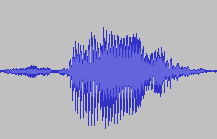
\includegraphics[width=1.25in]{images/start.png}}\\
    \end{center}
    Coefficients
  	\begin{itemize}
	\item -1.6538
	\item 1.0859
	\item -0.8826
	\item 0.3327
	\item 0.1480
  	\end{itemize}
	\end{block}
  \column{1.8in}
  	\begin{block}{``stop"}
  	\begin{center}
  	\frame{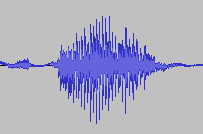
\includegraphics[width=1.25in]{images/stop.png}}\\
  	\end{center}
  	Coefficients
  	\begin{itemize}
  	\item -1.9805
	\item 1.7414
	\item -1.3340
	\item 0.5479
	\item 0.0415
  	\end{itemize}
	\end{block}
\end{columns}
\end{frame}

%------------------------------------------------

\begin{frame}
\frametitle{LPC Coefficients Extraction Method}
\begin{columns}[c]
  \column{2in}
    \begin{block}{Parameters}
    \begin{itemize}
    	\item $N$ - Number of desired coefficients per frame
		\item $S_f$ - Frame size in milliseconds
		\item $S_o$ - The overlap of frames in milliseconds
		\item Simply concatenate the coefficients from each frame together
    \end{itemize}
    \end{block}
  \column{1.8in}
  	\frame{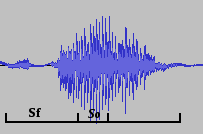
\includegraphics[width=2in]{images/lpc_parameters.png}}\\
\end{columns}
\end{frame}


%------------------------------------------------
\section{Classification}
%------------------------------------------------

\begin{frame}
\frametitle{Train Classifier}
\begin{columns}[c]
  \column{2.5in}
  	\begin{block}{Support Vector Machines (SVM)}
	\begin{itemize}
	\item Linearly separates complex feature space by projecting to a higher dimension
	\item Use radial basis kernel function $K(x, x') = \exp(\gamma||x-x'||^2))$
	\item 5 fold cross validation
	\item Grid search for cost function (C) and $\gamma$
	\end{itemize}
	\end{block}
  \column{1.5in}
	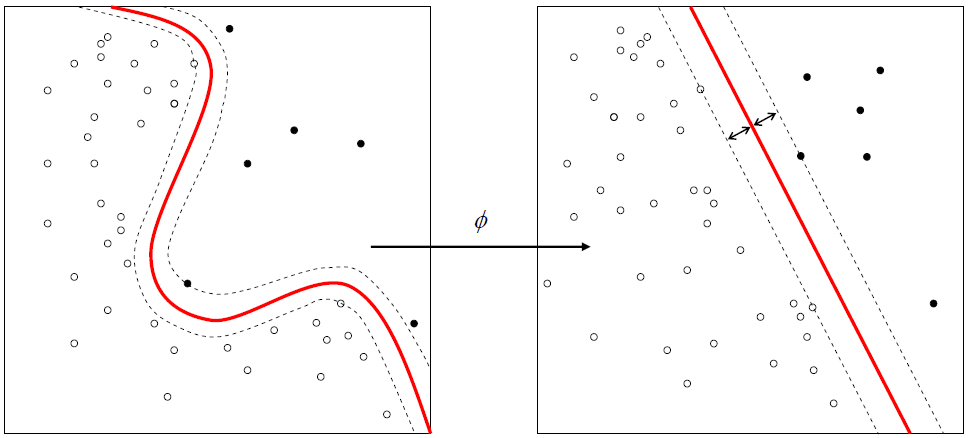
\includegraphics[width=1.5in]{images/svm.png}
	\\
	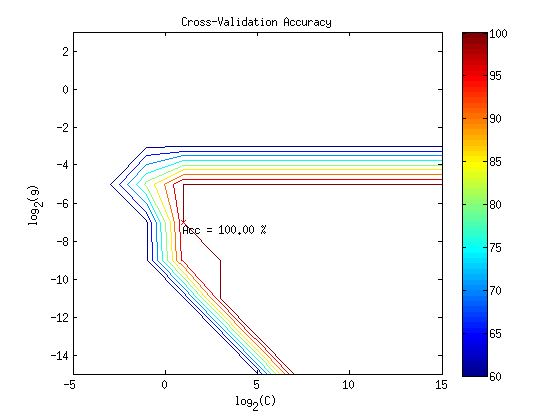
\includegraphics[width=1.5in]{images/grid.png}
\end{columns}
\end{frame}

%------------------------------------------------

\begin{frame}
\frametitle{Real Time Prediction}
  	\begin{block}{Continuously Loop}
	\begin{itemize}
	\item Record 2 seconds of audio
	\item Check for silence
	\item Calculate the LPC filter coefficients
	\item Pass the coefficient feature vector through the SVM classifier
	\item Output identified class
	\end{itemize}
	\end{block}
\end{frame}

%------------------------------------------------
\section{Examples}
%------------------------------------------------

\begin{frame}
\frametitle{Commands 
\href{images/commands.mp4}{
\includegraphics[width=0.15in]{images/play.png}}}
Simple commands for controlling a remote control vehicle.
\begin{columns}[c]
  \column{1.5in}
	\begin{block}{Vocabulary}
		\begin{itemize}
		\item Start
		\item Stop
		\item Left
		\item Right
		\end{itemize}
	\end{block}
  \column{2.5in}
  	\begin{block}{SVM}
		\begin{itemize}
		\item $N$ = 100
		\item $S_f$ = 60ms
		\item $S_o$ = 0ms
		\item 48 Training Samples
		\item 32 Verification Samples
		\item \small{Cross Validation Accuracy = 93.75\%}
		\item Verification Accuracy = 96.875\%
		\end{itemize}
	\end{block}
\end{columns}
\end{frame}

%------------------------------------------------

\begin{frame}
\frametitle{Piano 
\href{images/piano.mp4}{
\includegraphics[width=0.15in]{images/play.png}}}
The notes of the C major scale played on a piano.
\begin{columns}[c]
  \column{1.5in}
	\begin{block}{Vocabulary}
		\begin{itemize}
		\item C4
		\item D4
		\item E4
		\item F4
		\item G4
		\item A4
		\item B4
		\item C5
		\end{itemize}
	\end{block}
  \column{2.5in}
  	\begin{block}{SVM}
		\begin{itemize}
		\item $N$ = 100
		\item $S_f$ = 30ms
		\item $S_o$ = 15ms
		\item 96 Training Samples
		\item 64 Verification Samples
		\item \small{Cross Validation Accuracy = 100\%}
		\item Verification Accuracy = 100\%
		\end{itemize}
	\end{block}
\end{columns}
\end{frame}


%------------------------------------------------

\begin{frame}
\frametitle{Speaker Recognition 
\href{images/speaker.mp4}{
\includegraphics[width=0.15in]{images/play.png}}}
The spoken word ``test" for two speakers.
\begin{columns}[c]
  \column{1.5in}
	\begin{block}{Vocabulary}
		\begin{itemize}
		\item Speaker 1
		\item Speaker 2
		\end{itemize}
	\end{block}
  \column{2.5in}
  	\begin{block}{SVM}
		\begin{itemize}
		\item $N$ = 100
		\item $S_f$ = 60ms
		\item $S_o$ = 15ms
		\item 24 Training Samples
		\item 16 Verification Samples
		\item \small{Cross Validation Accuracy = 95.83\%}
		\item Verification Accuracy = 100\%
		\end{itemize}
	\end{block}
\end{columns}
\end{frame}

%------------------------------------------------

\begin{frame}
\frametitle{Simple Arithmetic 
\href{images/math.mp4}{
\includegraphics[width=0.15in]{images/play.png}}}
The symbols necessary for simple arithmetic.
\begin{columns}[c]
  \column{1.5in}
	\begin{block}{Vocabulary}
		\begin{itemize}
		\item 1, 2, 3, 4, 5,\\ 6, 7, 8, 9, 0
		\item $+, -, /, \times, =$
		\end{itemize}
	\end{block}
  \column{2.5in}
  	\begin{block}{SVM}
		\begin{itemize}
		\item $N$ = 100
		\item $S_f$ = 60ms
		\item $S_o$ = 30ms
		\item 300 Training Samples
		\item 60 Verification Samples
		\item \small{Cross Validation Accuracy = 96.67\%}
		\item Verification Accuracy = 98.33\%
		\end{itemize}
	\end{block}
\end{columns}
\end{frame}

%------------------------------------------------
\section{Conclusion}
%------------------------------------------------

\begin{frame}
\frametitle{Evaluation of Results and Future Work}
\begin{block}{}
\begin{itemize}
	\item Very susceptible to changes in environment
	\begin{itemize}
		\item Background noise
		\item Changes in location
		\item Changes in speaker
	\end{itemize}
	\item Significantly increase training database size
	\item Use other features in classification
	\begin{itemize}
		\item Fourier Transform
		\item Wavelet Transform
	\end{itemize}
	\item Create better real time prediction environment
\end{itemize}
\end{block}
\end{frame}

%------------------------------------------------

\begin{frame}
\frametitle{References}
\small{
\begin{thebibliography}{99}
\setbeamertemplate{bibliography item}[text]
\bibitem{E}
C.Senthilkumar. ``Maximizing the Speech Recognition Accuracy Using Linear predictive Coding'' [Online] Available: \url{http://www.academia.edu/4874338/Maximizing_the_Speech_Recognition_Accuracy_Using_Linear_predictive_Coding_Guided_by_Maximizing_the_Speech_Recognition_Accuracy_Using_Linear_predictive_Coding}\\

\bibitem{E}
E. Doering. ``Linear Prediction and Cross Synthesis'' [Online] Available: \url{https://legacy.cnx.org/content/m15478/latest/}

\bibitem{E}
T. Wijoyo, S. Wijoyo. ``Speech Recognition Using Linear Predictive Coding and Artificial Neural Network for Controlling Movement of Mobile Robot'' [Online] Available: \url{www.ipcsit.com/vol6/36-E091.pdf}

\bibitem{E}
U. Shrawankar. ``Techniques for Feature Extraction in Speech
Rcognition System : A Comparative Study'' [Online] Available: \url{http://arxiv.org/ftp/arxiv/papers/1305/1305.1145.pdf}

\end{thebibliography}
}


\end{frame}

%------------------------------------------------

\begin{frame}
\Huge{\centerline{Questions?}}
\end{frame}

%----------------------------------------------------------------------------------------

\end{document} 